\documentclass[12pt, a4paper]{article}

% Encoding and language
\usepackage[utf8]{inputenc}
\usepackage[T1]{fontenc}
\usepackage[spanish]{babel}

% Layout
\usepackage[margin=2.5cm]{geometry}
\usepackage{parskip}
\usepackage{setspace}
\onehalfspacing

% Math and code
\usepackage{amsmath}
\usepackage{listings}
\usepackage{xcolor}

% Tables and figures
\usepackage{booktabs}
\usepackage{graphicx}
\usepackage{float}
\usepackage{caption}
\usepackage{subcaption}
\usepackage{array}
\usepackage{multirow}

% Links
\usepackage[hidelinks]{hyperref}

% Header / footer
\usepackage{fancyhdr}
\setlength{\headheight}{15pt}
\pagestyle{fancy}
\fancyhf{}
\lhead{\small Minería de Datos — Práctica 3.6}
\rhead{\small Equipo 10}
\cfoot{\thepage}
\renewcommand{\headrulewidth}{0.4pt}

% Code style
\lstdefinestyle{python}{
  language=Python,
  basicstyle=\ttfamily\small,
  keywordstyle=\color{blue!70!black}\bfseries,
  commentstyle=\color{gray},
  stringstyle=\color{teal},
  showstringspaces=false,
  breaklines=true,
  frame=single,
  backgroundcolor=\color{gray!6},
  rulecolor=\color{gray!30},
  numbers=left,
  numberstyle=\tiny\color{gray},
  numbersep=8pt,
}

% ─────────────────────────────────────────────
\begin{document}

% ── Portada ───────────────────────────────────
\begin{titlepage}
  \centering
  \vspace*{1.5cm}

  {\Large\bfseries Universidad Nacional Autónoma de México\\[0.3em]
  Facultad de Ingeniería}\\[0.8em]
  {\large Minería de Datos}

  \vspace{2cm}
  \rule{\linewidth}{0.6pt}\\[0.6em]
  {\LARGE\bfseries Práctica 3.6\\[0.4em]
  Redes Neuronales Convolucionales (CNN)\\[0.3em]
  \large Reconocimiento de Emociones Faciales con FER-2013}\\[0.4em]
  \rule{\linewidth}{0.6pt}

  \vspace{2cm}

  {\large\textbf{Equipo 10}}\\[0.5em]
  {\large Prof. Jose Roberto Olvera Lopez}\\[1.5em]

  \vspace{2cm}

  {\large Mayo 2026}

  \vfill
  {\small Archivos del proyecto disponibles en: \url{https://github.com/e1th4nUwU/CNN-FER2013-Example}}
\end{titlepage}

% ── Índice ────────────────────────────────────
\tableofcontents
\newpage

% ─────────────────────────────────────────────
\section{Propósito de la Práctica}

\subsection{Contexto: Estudio Original}

En 2020, Sturm et al.\ (UCSF) publicaron un ensayo clínico aleatorizado con 60 adultos mayores
(60–90 años) en el que evaluaron si caminatas breves diseñadas para cultivar \textbf{asombro}
(\textit{awe}) podían mejorar el bienestar emocional \cite{sturm2022}. Durante ocho semanas,
los participantes tomaban tres \textit{selfies} por caminata —1,184 fotos en total— y respondían
encuestas de estado emocional al terminar cada sesión.

Para analizar los cambios conductuales en las fotografías, los autores emplearon MATLAB Image
Processing Toolbox: binarizaron cada imagen en píxeles ``yo'' vs.\ ``fondo'' y calcularon el
\textit{self-size} —qué proporción del encuadre ocupa la persona— como indicador indirecto de
auto-enfoque. Adicionalmente, codificaron \textbf{manualmente} la intensidad de sonrisa en cada
foto. Los resultados mostraron que los participantes del grupo \textit{awe} progresivamente
cedieron más espacio al entorno y sonrieron con mayor intensidad semana a semana.

\subsection{Caso de Negocio}

El protocolo del estudio original presenta dos limitaciones prácticas:

\begin{enumerate}
  \item \textbf{Escalabilidad}: la codificación manual de sonrisas es costosa y subjetiva;
        MATLAB requiere umbralización artesanal por sesión.
  \item \textbf{Riqueza emocional}: el \textit{self-size} captura comportamiento de encuadre,
        no emoción directamente; la codificación manual solo distingue intensidad de sonrisa,
        sin mapear el espectro emocional completo.
\end{enumerate}

Una extensión natural del estudio consistiría en \textbf{reemplazar ambas métricas por un
clasificador automático de expresiones faciales}. Este clasificador permitiría:

\begin{itemize}
  \item Rastrear trayectorias emocionales longitudinales (semana 1 $\to$ semana 8) de forma automática.
  \item Comparar la distribución de emociones entre el grupo \textit{awe} y el grupo control.
  \item Probar la hipótesis de que el grupo \textit{awe} exhibirá un incremento progresivo en
        clasificaciones \texttt{happy} y una reducción en \texttt{neutral}/\texttt{sad}.
  \item Escalar el protocolo a estudios con mayor número de participantes sin costo analítico proporcional.
\end{itemize}

Las 1,184 selfies recopiladas en el estudio original no están disponibles públicamente —los
participantes son adultos mayores y los datos permanecen bajo resguardo por consideraciones
éticas y de privacidad—. Por ello, este trabajo entrena el clasificador sobre el dataset público
\textbf{FER-2013} como \textit{proxy}. FER-2013 ofrece la misma tarea de clasificación (7 emociones,
imágenes de rostros en condiciones variables) y permite validar la arquitectura antes de su
eventual aplicación sobre el corpus del estudio.

\subsection{Objetivo Técnico}

Entrenar una Red Neuronal Convolucional (CNN) capaz de clasificar imágenes de rostros humanos
en \textbf{7 categorías de emoción}: \textit{angry}, \textit{disgust}, \textit{fear},
\textit{happy}, \textit{neutral}, \textit{sad} y \textit{surprise}.

% ─────────────────────────────────────────────
\section{Pasos Realizados y Parámetros Seleccionados}

\subsection{Dataset: FER-2013}

\begin{table}[H]
  \centering
  \caption{Características del dataset FER-2013}
  \begin{tabular}{ll}
    \toprule
    \textbf{Atributo} & \textbf{Valor} \\
    \midrule
    Fuente            & Kaggle — \texttt{msambare/fer2013} \\
    Total de imágenes & $\approx$35,000 \\
    Conjunto de entrenamiento & 28,709 imágenes \\
    Conjunto de prueba        & 7,178 imágenes \\
    Resolución        & 48×48 px, escala de grises \\
    Clases            & 7 (angry, disgust, fear, happy, neutral, sad, surprise) \\
    \bottomrule
  \end{tabular}
\end{table}

\subsection{Preprocesamiento y Aumento de Datos}

Las imágenes se normalizaron dividiéndolas entre 255 para escalar los píxeles al rango $[0,1]$.
Para el conjunto de entrenamiento se aplicó aumento de datos con el objetivo de mejorar la
generalización del modelo y reducir el sobreajuste:

\begin{lstlisting}[style=python]
train_datagen = ImageDataGenerator(
    rescale=1./255,
    rotation_range=10,
    width_shift_range=0.1,
    height_shift_range=0.1,
    horizontal_flip=True,
    zoom_range=0.1
)
test_datagen = ImageDataGenerator(rescale=1./255)
\end{lstlisting}

El conjunto de prueba solo recibe normalización, sin transformaciones aleatorias, para garantizar
una evaluación reproducible.

\subsection{Arquitectura de la CNN}

La red se compone de tres bloques convolucionales seguidos de capas de clasificación:

\begin{table}[H]
  \centering
  \caption{Arquitectura de la CNN}
  \begin{tabular}{llr}
    \toprule
    \textbf{Capa} & \textbf{Configuración} & \textbf{Parámetros} \\
    \midrule
    Conv2D (bloque 1)        & 32 filtros, kernel 3×3, ReLU  & 320 \\
    BatchNormalization        & —                             & 128 \\
    MaxPooling2D              & pool 2×2                      & 0   \\
    Conv2D (bloque 2)        & 64 filtros, kernel 3×3, ReLU  & 18,496 \\
    BatchNormalization        & —                             & 256 \\
    MaxPooling2D              & pool 2×2                      & 0   \\
    Conv2D (bloque 3)        & 128 filtros, kernel 3×3, ReLU & 73,856 \\
    BatchNormalization        & —                             & 512 \\
    MaxPooling2D              & pool 2×2                      & 0   \\
    Flatten                   & —                             & 0   \\
    Dense                     & 256 unidades, ReLU            & 524,544 \\
    Dropout                   & tasa = 0.5                    & 0   \\
    Dense (salida)            & 7 unidades, Softmax           & 1,799 \\
    \midrule
    \multicolumn{2}{l}{\textbf{Total parámetros entrenables}} & \textbf{619,463} \\
    \bottomrule
  \end{tabular}
\end{table}

\subsection{Compilación y Entrenamiento}

\begin{lstlisting}[style=python]
model.compile(
    optimizer='adam',
    loss='categorical_crossentropy',
    metrics=['accuracy']
)
model.fit(train_generator, epochs=50,
          validation_data=test_generator, callbacks=callbacks)
\end{lstlisting}

\begin{itemize}
  \item \textbf{Optimizador}: Adam — adapta la tasa de aprendizaje por parámetro, acelerando
        la convergencia en clasificación de imágenes.
  \item \textbf{Función de pérdida}: \texttt{categorical\_crossentropy} — apropiada para
        clasificación multiclase con etiquetas \textit{one-hot encoded}.
  \item \textbf{Épocas máximas}: 50 (controladas por \textit{callbacks}).
  \item \textbf{Tamaño de lote}: 64.
\end{itemize}

\subsubsection{Callbacks de Entrenamiento}

Se utilizaron tres \textit{callbacks} para mejorar la calidad del entrenamiento:

\begin{table}[H]
  \centering
  \caption{Callbacks configurados}
  \begin{tabular}{p{3.5cm}p{4.5cm}p{5.5cm}}
    \toprule
    \textbf{Callback} & \textbf{Parámetros clave} & \textbf{Función} \\
    \midrule
    \texttt{ModelCheckpoint} &
      \texttt{monitor='val\_accuracy'},\newline\texttt{save\_best\_only=True} &
      Guarda \texttt{best\_model.keras} cada vez que \texttt{val\_accuracy} mejora. \\
    \addlinespace
    \texttt{ReduceLROnPlateau} &
      \texttt{factor=0.5},\newline\texttt{patience=3},\newline\texttt{min\_lr=1e-6} &
      Reduce el learning rate a la mitad si \texttt{val\_loss} no mejora en 3 épocas consecutivas. \\
    \addlinespace
    \texttt{EarlyStopping} &
      \texttt{patience=8},\newline\texttt{restore\_best\_weights=True} &
      Detiene el entrenamiento si \texttt{val\_loss} no mejora en 8 épocas; restaura los mejores pesos. \\
    \bottomrule
  \end{tabular}
\end{table}

% ─────────────────────────────────────────────
\section{Resultados Obtenidos}

\subsection{Métricas Globales}

El modelo alcanzó una \textbf{precisión global de 63.03\%} en el conjunto de prueba
(pérdida: 0.9993).

\subsection{Reporte de Clasificación por Clase}

\begin{table}[H]
  \centering
  \caption{Métricas de clasificación por emoción}
  \begin{tabular}{lrrrr}
    \toprule
    \textbf{Emoción} & \textbf{Precisión} & \textbf{Recall} & \textbf{F1-Score} & \textbf{Soporte} \\
    \midrule
    Angry    & 0.52 & 0.58 & 0.55 & 958  \\
    Disgust  & 0.80 & 0.18 & 0.29 & 111  \\
    Fear     & 0.49 & 0.32 & 0.38 & 1024 \\
    Happy    & 0.85 & 0.86 & 0.85 & 1774 \\
    Neutral  & 0.56 & 0.69 & 0.62 & 1233 \\
    Sad      & 0.49 & 0.50 & 0.50 & 1247 \\
    Surprise & 0.76 & 0.77 & 0.76 & 831  \\
    \midrule
    \textbf{Macro avg}    & 0.64 & 0.55 & 0.56 & 7178 \\
    \textbf{Weighted avg} & 0.63 & 0.63 & 0.62 & 7178 \\
    \bottomrule
  \end{tabular}
\end{table}

\subsection{Curvas de Entrenamiento}

\begin{figure}[H]
  \centering
  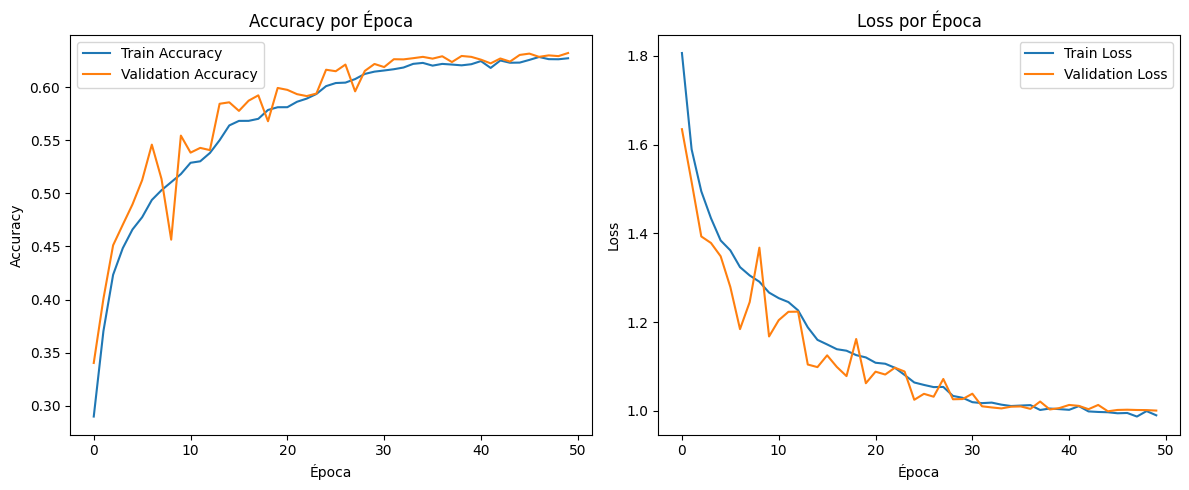
\includegraphics[width=0.9\textwidth]{img/accuracy-and-loss.png}
  \caption{Accuracy y Loss por época durante el entrenamiento}
  \label{fig:training-curves}
\end{figure}

\subsection{Matriz de Confusión}

\begin{figure}[H]
  \centering
  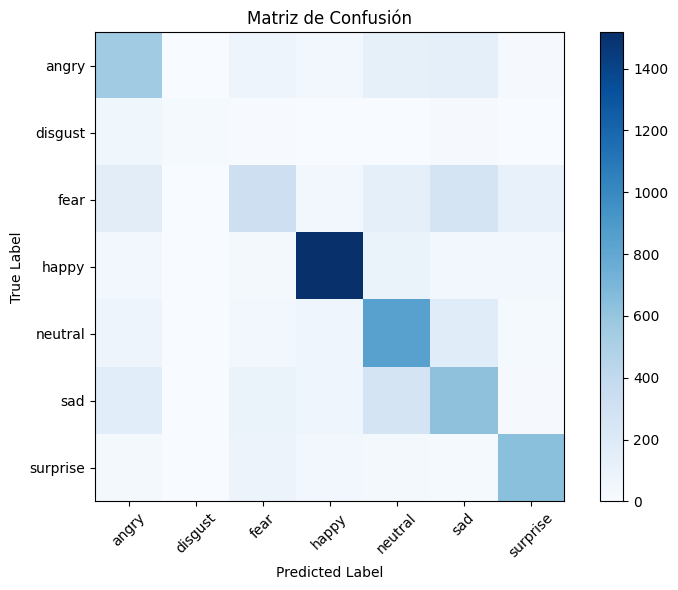
\includegraphics[width=0.65\textwidth]{img/confusion-matrix.png}
  \caption{Matriz de confusión sobre el conjunto de prueba}
  \label{fig:confusion-matrix}
\end{figure}

% ─────────────────────────────────────────────
\section{Conclusiones}

\subsection{Rendimiento por clase}

El modelo alcanzó una precisión global de 63\% sobre FER-2013, con desempeño muy
dispar entre clases. \textit{Happy} obtuvo el mejor resultado (F1 = 0.85) gracias a
sus rasgos faciales altamente distintivos. \textit{Surprise} también mostró buen
desempeño (F1 = 0.76). En contraste, \textit{disgust} obtuvo el F1 más bajo (0.29)
debido a un severo desbalance de clases: solo 111 muestras de prueba frente a 1,774
de \textit{happy}.

\subsection{Emociones más difíciles}

Las emociones \textit{fear} y \textit{sad} presentaron los menores rendimientos
(F1 = 0.38 y 0.50, respectivamente) por dos razones complementarias: comparten
microexpresiones faciales similares —comisuras hacia abajo, tensión en cejas—, y el
desbalance de clases impide al modelo aprender representaciones suficientemente
discriminativas para \textit{disgust}.

\subsection{Relevancia para el caso de negocio}

Desde la perspectiva de Sturm et al., el resultado más importante es que
\textit{happy} —la emoción central del protocolo de \textit{awe walks}— alcanza
F1 = 0.85, validando la utilidad del clasificador para rastrear trayectorias
emocionales longitudinales. El buen desempeño en \textit{surprise} (F1 = 0.76)
también es relevante, ya que el asombro se manifiesta frecuentemente como una
combinación de felicidad y sorpresa. El bajo rendimiento en \textit{disgust} y
\textit{fear} no representa un obstáculo crítico, pues esas emociones no son las
hipótesis de interés del estudio.

\subsection{Mejoras propuestas}

\begin{enumerate}
  \item \textbf{Balanceo de clases}: aplicar \textit{oversampling} (SMOTE o aumento
        de datos agresivo) sobre las clases minoritarias, particularmente
        \textit{disgust}.
  \item \textbf{Transfer learning}: reemplazar la arquitectura desde cero por un
        modelo pre-entrenado (VGG16, EfficientNetB0) con \textit{fine-tuning}. En
        FER-2013, estas arquitecturas alcanzan 70–75\% de accuracy.
  \item \textbf{Adaptación al dominio}: el corpus del estudio consiste en selfies de
        adultos mayores en exteriores, dominio diferente al de FER-2013. Un ciclo de
        \textit{domain adaptation} o fine-tuning sobre una pequeña muestra anotada
        mejoraría significativamente el desempeño en producción.
  \item \textbf{Umbrales de confianza por clase}: en producción, usar umbrales
        diferenciados para rechazar predicciones de baja confianza en clases como
        \textit{fear} y \textit{disgust}.
\end{enumerate}

% ─────────────────────────────────────────────
\begin{thebibliography}{9}

\bibitem{sturm2022}
Sturm, V.\ E., Datta, S., Roy, A.\ R.\ K., Sible, I.\ J., Kosik, E.\ L., Veziris, C.\ R.,
Chow, T.\ E., Morris, N.\ A., Neuhaus, J., Kramer, J.\ H., Miller, B.\ L., Holley, S.\ R.,
\& Keltner, D.\ (2022).
\textit{Big smile, small self: Awe walks promote prosocial positive emotions in older adults.}
\textit{Emotion}, 22(5), 1044–1058.
\url{https://doi.org/10.1037/emo0000876}

\bibitem{fer2013}
Goodfellow, I.\ J., Erhan, D., Carrier, P.\ L., Courville, A., Mirza, M., Hamner, B.,
Cukierski, W., Tang, Y., Thaler, D., Lee, D.-H., Zhou, Y., Ramaiah, C., Feng, F., Li, R.,
Wang, X., Athanasakis, D., Shawe-Taylor, J., Milakov, M., Park, J., \ldots\ Bengio, Y.\
(2013).
\textit{Challenges in Representation Learning: A Report on Three Machine Learning Contests.}
arXiv:1307.0414.

\bibitem{fer2013-kaggle}
Sambare, M.\ (2020).
\textit{FER-2013} [Dataset].
Kaggle.
\url{https://www.kaggle.com/datasets/msambare/fer2013}

\bibitem{lecun1989}
LeCun, Y., Boser, B., Denker, J.\ S., Henderson, D., Howard, R.\ E., Hubbard, W.,
\& Jackel, L.\ D.\ (1989).
\textit{Backpropagation applied to handwritten zip code recognition.}
\textit{Neural Computation}, 1(4), 541–551.

\bibitem{tensorflow}
Abadi, M., et al.\ (2015).
\textit{TensorFlow: Large-scale machine learning on heterogeneous systems.}
\url{https://www.tensorflow.org}

\end{thebibliography}

\end{document}
